\section{Project Objectives}
The primary objectives of this project are:

\begin{itemize}
	\item To design and implement a two-wheeled self-balancing mobile platform capable of maintaining dynamic stability using real-time sensor feedback and control algorithms.
	\item To develop a robust control framework that ensures precise balancing and smooth motion control, with resilience to external disturbances.
	\item To integrate an Inertial Measurement Unit (IMU) and Hall-effect rotary encoders, utilizing sensor fusion techniques such as the Kalman filter, to achieve accurate state estimation, including orientation and velocity.
	\item To enhance the robot’s spatial awareness through 2D environmental mapping using Time-of-Flight (ToF) sensors.
	\item To develop a central communication and control hub, facilitating data integration between the mobile base, ToF sensors, and external systems, enabling real-time monitoring and remote control over Wi-Fi.
	\item To provide comprehensive documentation of the system design, control strategies, and software implementation, and to openly share the source code and resources via GitHub to support reproducibility and future development.
\end{itemize}



\section{Literature Review}
Wheeled robots are inherently more efficient than bipedal counterparts due to their lower energy consumption, simpler mechanics, and reduced control complexity. This makes them not only more cost-effective to produce and maintain but also highly suitable for structured indoor environments where agility and compactness are essential \cite{bjelonic_survey_2023}. Today, robots are used in a variety of environments beyond industrial and clinical settings, including everyday locations such as offices, hotels, hospitals, and homes, where they frequently interact with people. In these situations, mobile robots frequently need to manoeuvrer effectively within limited spaces \cite{kim2010practical}. Therefore, a two-wheeled robot was selected for the mobile base for this research project. The \href{https://www.elegoo.com/products/elegoo-tumbller-self-balancing-robot-car}{ELEGOO Tumbler} (shown in Fig. \ref{fig:tumbler}) was selected as a base platform, as it provides nearly all the necessary hardware in a convenient DIY kit.

\begin{figure}[h]
	\centering
	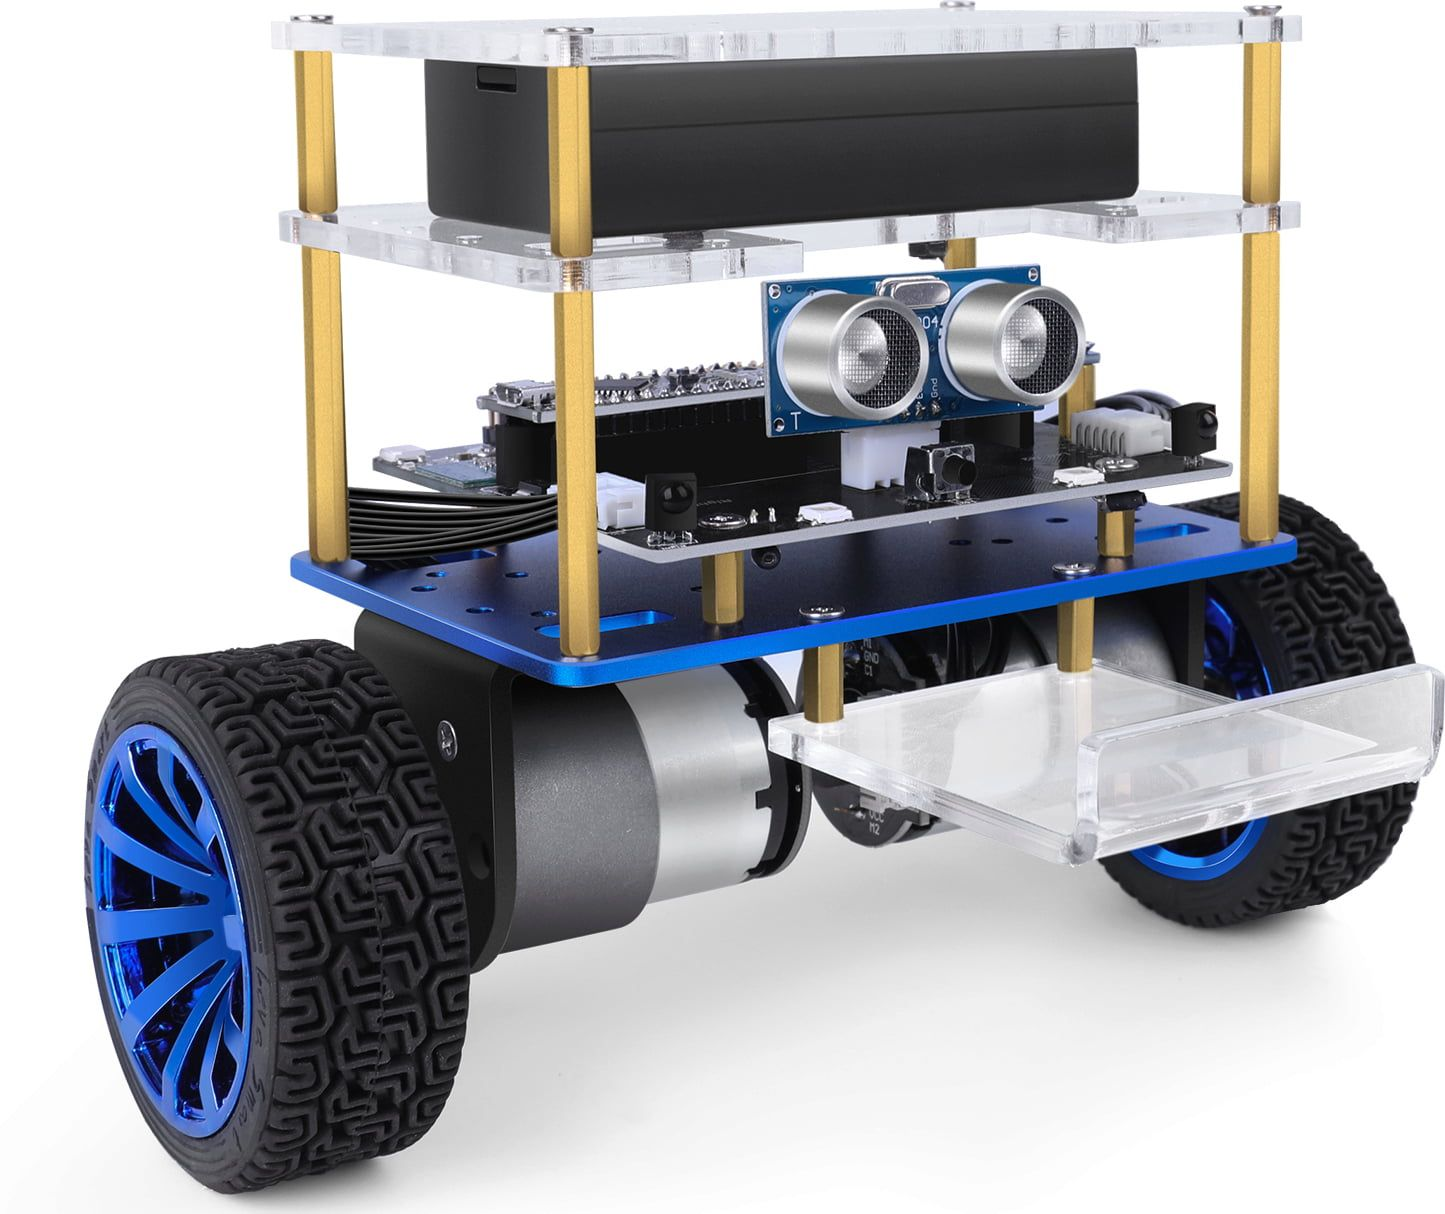
\includegraphics[height=6cm]{assets/tumbller.jpg}
	\caption{\label{fig:tumbler} ELEGOO Tumbler used as the mobile base for this project~\cite{tumbller}.}
\end{figure}

Two-wheeled self-balancing robots have been widely studied as a variant of the classic inverted pendulum problem, requiring control strategies to maintain stability. Various approaches, including Proportional-Integral-Derivative (PID) control \cite{matlab_inverted_pendulum}, Lead-Lag~\cite{nise2020control} and Fuzzy Control~\cite{passino1998fuzzy} have been explored to achieve robust balancing and motion control. Abdelgawad et al.~\cite{abdelgawad2024model} demonstrated that PID control offers higher accuracy, lower error, faster response, and greater robustness, while also being easier to tune—making it well-suited for precise control applications. Kalman filter \cite{kalman1960new} has been shown to significantly enhance state estimation accuracy \cite{IJRCS1674, ngo2017experimental, 7334442}, and is therefore also employed in this project. 

This project, we aim to develop a lightweight and efficient system for 2D environmental mapping in compact indoor settings. For Time-of-Flight (ToF) sensing, the Terabee TeraRanger Multiflex (shown in Fig.~\ref{fig:terraMount}) was selected due to its reliable range of up to 2 meters and its modular design featuring eight pre-calibrated, plug-and-play sensors~\cite{TeraRanger2025}. These characteristics make it particularly well-suited for applications that require low power consumption and scalability. The ESP32-S3-DevKitC-1 (shown in Fig.\ref{fig:ESP32-Photo}) was similarly selected as the communication hub for its open-source support, integrated Wi-Fi, and dual-core processing~\cite{ESP32-S3-DevKitC-1}. These capabilities enable efficient real-time data handling and peripheral communication, which are critical for processing input from the sensors and forwarding.

\begin{figure}[h]
	\centering
	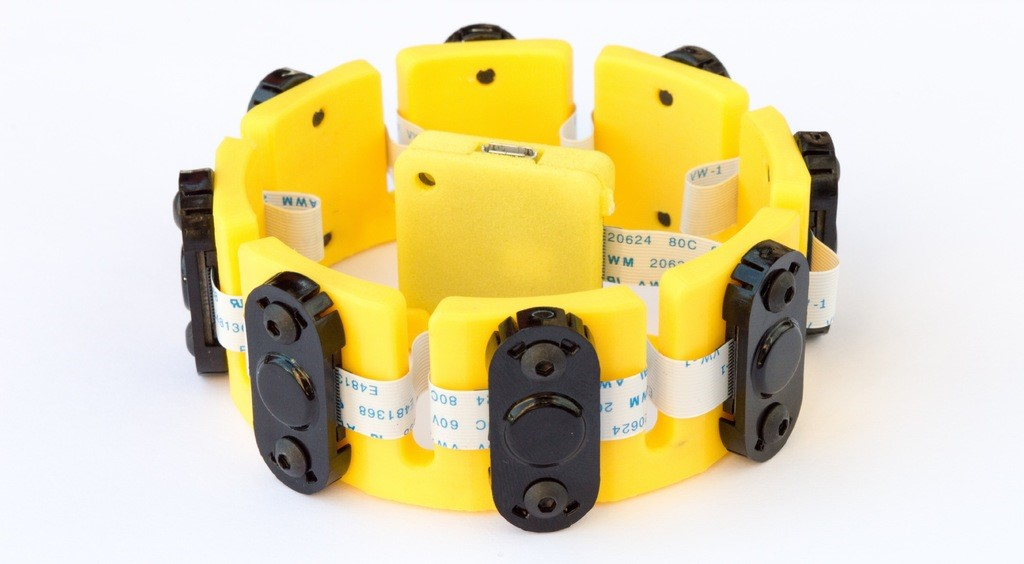
\includegraphics[height=6cm]{assets/terraRangerMultiplex.jpg}
	\caption{TeraRanger Multiflex circular mount \cite{terra_mount}.}
	\label{fig:terraMount}
\end{figure}

\begin{figure}[h]
	\centering
	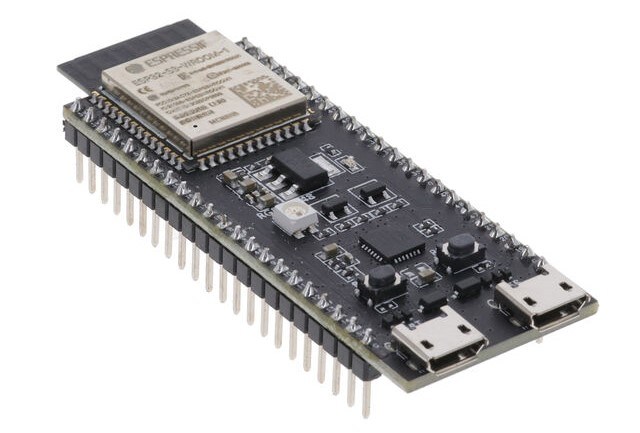
\includegraphics[height=3.2cm]{assets/ESP32-S3-DEVKITC-1-N8R8.jpg}
	\caption{ESP32-S3-DevKitC-1-N8R8 from Espressif Systems\cite{ESP32-S3-DevKitC-1-Photo-Datasheet}.}
	\label{fig:ESP32-Photo}
\end{figure}